
\section{泛基因组学(Pan-genome):内容、应用场景、研究实例}
泛基因组代表了一个物种内的所有基因集合,由核心基因组(包含物种所有个体间共享的序列)和“可选”基因组组成.2005年,泛基因组这一概念首次应用于细菌物种研究\cite{tettelin2005genome},当时在对数株链球菌(Streptococcus agalactiae)的测序中发现,核心基因组包含了80\%的链球菌基因,而其余20\%的基因在至少一个菌株中缺失.从那时起,研究人员一直在努力揭示许多物种的泛基因组,如2010年进行的人类泛基因组研究\cite{li2009human}.泛基因组研究表明,依赖于单一的参考基因组可能会对我们对物种多样性的理解产生负面影响.例如,在植物物种中\cite{Bayer2020PlantPA},与农艺性状相关的许多重要基因通常位于可选基因组中.随着基因组测序技术的不断改进,特别是长读取测序的发展,研究者们开始构建更复杂物种的泛基因组.通过泛基因组研究,我们发现单一参考基因组无法充分代表物种内群体的遗传多样性,因此泛基因组研究在未来植物育种、疾病抗性和环境适应性等方面具有广泛的应用前景.

\subsection{内容}
泛基因组(pangenome 或 supragenome)是指分类单元(clade)内所有菌株(strains, 实际上也可以推广到物种)的所有基因集合.它可分为核心泛基因组(core pangenome,所有个体中存在的基因)、壳层泛基因组(shell pangenome,两个或更多菌株中存在的基因)和云泛基因组(cloud pangenome,仅在单个菌株中发现的基因),如图\ref{Parts_of_the_pangenome}中所示.云基因组也称为附属基因组,包含部分菌株中存在的可有可无的基因和菌株特异性基因.研究泛基因组的领域称为泛基因组学.

\begin{figure}[htp!]
	\centering
	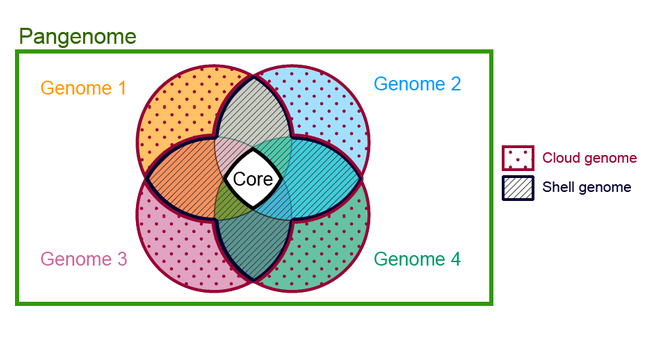
\includegraphics[width=1\linewidth]{figure/Parts_of_the_pangenome}
	\caption{泛基因组中的不同类型} \label{Parts_of_the_pangenome}
\end{figure}


细菌物种的基因组比单个菌株的基因含量大得多.有些物种具有开放泛基因组,而另一些具有封闭泛基因组.人口规模和生态位多样性被认为是决定泛基因组大小的主要因素.
泛基因组最初为细菌和古菌物种构建,近年来发展了真核生物泛基因组,特别是植物物种.泛基因组动态与可移动元件有关,具有重要的进化背景意义,与宏基因组学相关,也在更广泛的基因组学背景中使用.


\begin{figure}[htp!]
	\centering
	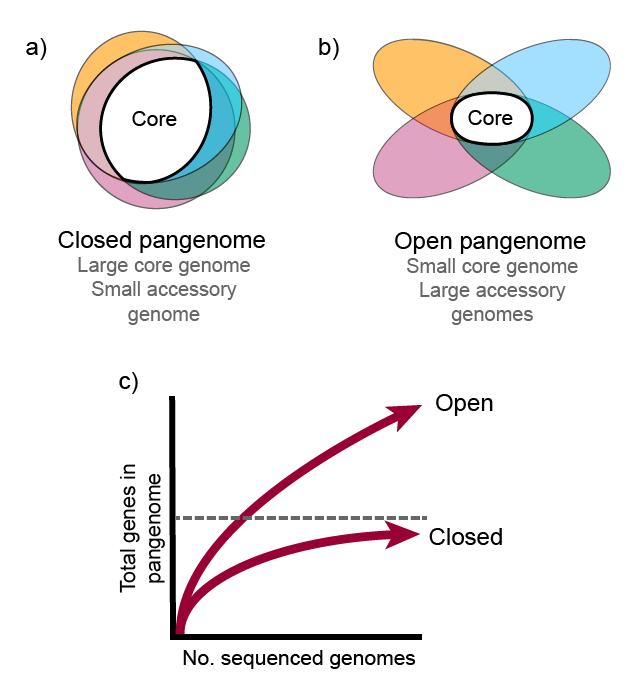
\includegraphics[width=0.55\linewidth]{figure/open_close}
	\caption{封闭和开放泛基因组.封闭泛基因组趋于渐近,可以预测完整大小.} \label{open_close}
\end{figure}

\subsection{应用场景}

想要深入理解泛基因组学的应用场景首先得明白泛基因组学的优点.泛基因组学的优点在于它能够更全面地揭示物种内的基因组多样性,揭示了整个基因组在不同物种中的重要性.因此,泛基因组学为我们提供了一个更全面的视角来研究物种内的遗传多样性,并为发掘有益基因提供了丰富的资源.



\subsubsection{作物基因组学、育种和进化研究}

泛基因组可以支持植物育种和进化研究,探讨基因存在和缺失变异的起源.第一个植物泛基因组研究是基于七个野生大豆个体的全基因组对比,发现与种子成分、开花和成熟时间、器官大小和生物量相关的可变基因以及在野生大豆Glycine soja中存在、而在家养大豆Glycine max中不存在的病害抗性基因\cite{li2014novo}.另一个研究基于三个不同水稻品种,发现一个栽培品种中S5杂种不育座位的缺失以及Sub1A水生状耐受基因的PAV\cite{schatz2014whole}.

\subsubsection{研究不同品种结构变异影响基因差异表达}

结构变异会影响基因的转录调控和表达,例如基因剂量变化、可变剪接和转录调控因子结合位点的改变.大豆泛基因组研究中,研究者通过对26个具有代表性的野生和栽培大豆品种进行de novo基因组组装,构建了一个高质量的基于图的大豆泛基因组.这一研究揭示了许多通过短序列直接映射到单一参考基因组上难以发现的遗传变异.基于图谱基因组的2,898个加入物的结构变异和来自代表性的26个加入物的RNA测序(RNA-seq)数据有助于将遗传变异与负责重要性状的候选基因联系起来.这一泛基因组资源将促进大豆的进化和功能基因组学研究.\cite{liu2020pan}.

\subsubsection{结合GWAS数据捕获更完整的遗传变异信息}

通过将泛基因组应用于GWAS分析,研究人员可以更全面地了解植物基因组的多样性,从而有助于揭示与重要性状相关的遗传变异,推动植物遗传改良和功能基因组学研究.传统GWAS分析在缺失参考基因组中的功能基因时,可能无法准确关联表型.然而,采用泛基因组作为参考,将结构变异纳入GWAS分析,有助于解决这一问题.

以一项关于油菜(Brassica napus)的研究\cite{song2020eight}为例,研究者通过测序、de novo组装和注释8个油菜品种,揭示了大量小型变异和存在及缺失变异(PAV).PAV基因组广泛关联研究(PAV-GWAS)成功确定了与籽荚长度、种子重量和开花时间相关的因果结构变异,这些变异在基于单核苷酸多态性的GWAS(SNP-GWAS)中未被检测到.此研究表明,PAV-GWAS可补充SNP-GWAS,识别与性状相关的关联,并为深入了解油菜基因组结构和遗传改良提供资源.

\subsection{研究实例:亚洲稻米泛基因组倒位指数}
下面,我将介绍一篇关于亚洲稻米泛基因组学研究的文章.这篇文章于2023年3月发表在《Nature Communications》上,题目为“亚洲水稻亚种群结构中泛基因组倒位指数揭示的进化启示”(Pan-genome inversion index reveals evolutionary insights into the subpopulation structure of Asian rice)\cite{zhou2023pan}.本文的主要作者是Yong Zhou等人,来自KAUST等多个机构.这项研究旨在探索亚洲稻米的基因多样性,并通过泛基因组学方法提供进化方面的见解.

\subsubsection{研究背景和内容}

为了应对2060年至2070年预期将达到100亿的全球人口增长,稻米研究社区正寻求创新方法,培育出营养丰富、可持续、能适应气候变化的新品种.在亚洲稻米的基因组中,有一些基因片段的顺序与其他个体不同,这种现象被称为倒位(inversion)\cite{rice}.倒位是一种重要的基因组结构变异,它可以影响基因的表达和功能.

本研究使用了73个高质量亚洲水稻(Oryza sativa)基因组,覆盖其亚种群结构,以及2个野生近缘种(O. rufipogon和O. punctata).研究人员基于这些基因组构建了一个包含1769个非冗余倒位的泛基因组倒位指数,涵盖了约29%的O. sativa cv. Nipponbare参考基因组序列.

通过该倒位指数,研究者估计亚洲水稻倒位发生率约为每百万年700次,这一速率是以往植物研究估算的16至50倍.对这些倒位的详细分析表明,它们对基因表达、重组率和连锁不平衡具有显著影响.该研究揭示了亚洲水稻泛基因组中大型倒位(≥100 bp)的普遍性和规模,并暗示了其在功能生物学和作物性状方面尚未充分研究的潜在影响.

\subsubsection{水稻倒位指数概述}

图\ref{invsum}中,$\mathbf{a}, \mathbf{b}$ 代表重采样置换检验,用于确定基因组数量与所有倒位和非基因组特异性倒位之间的关系;$ \mathbf{c} $ 倒位区域密度;$ \mathbf{d} $ Bionano对大于1 Mb的倒位进行验证,即Clu-INV0100180,Clu-INV0100660和Clu-INV0600550.在每个面板中,顶部线条显示作为参考的光学图谱,底部线条显示具有倒位的品种的基因组组装.灰色线条连接对齐的限制位点(蓝色区域),而黄色片段显示未对齐区域.黑色框突出显示每个倒位的位置.源数据作为源数据文件提供.

\begin{figure}[htp!]
	\centering
	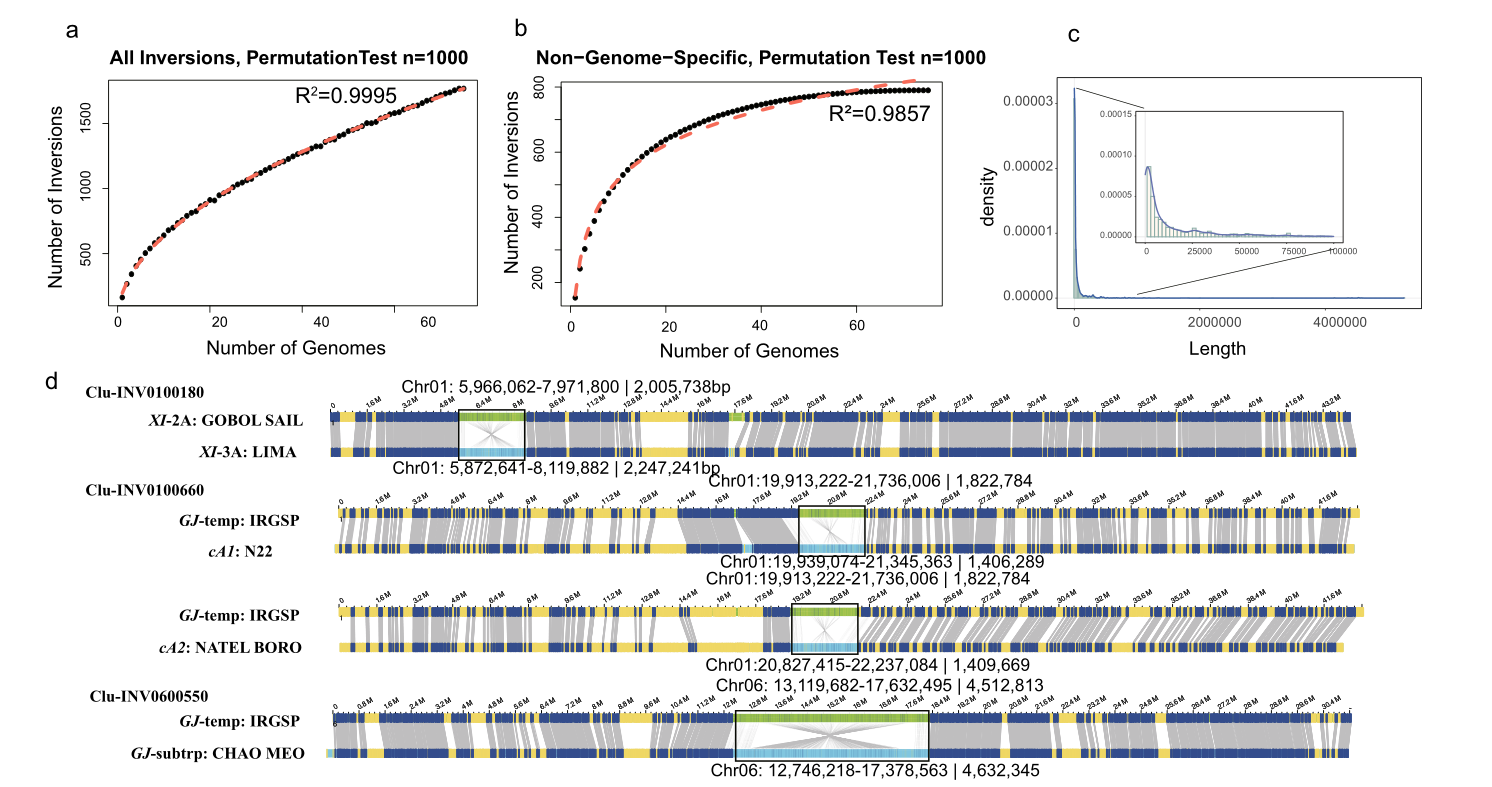
\includegraphics[width=1\linewidth]{figure/invsum}
	\caption{水稻倒位指数概述图} \label{invsum}
\end{figure}

这部分中,研究人员使用了一些典型的数据处理方法:

\begin{enumerate}
	\item 重采样置换检验(Resampling permutation test):这是一种统计方法,通过对数据进行随机重新排列,来评估观察到的结果是否具有显著性.在本研究中,研究者使用重采样置换检验来确定基因组数量与所有倒位和非基因组特异性倒位之间的关系.
	
	在 $ n $ 次置换后,对于重采样置换检验的 $ p $ 值计算可使用以下公式:
	$$
	p=\frac{1+\sum_{i=1}^n I\left(T_i \geq T_{o b s}\right)}{n+1}
	$$
	其中, $I$ 是示性函数,$ T_i $ 表示第 $ i $ 次置换的统计 量,$T_{obs}$表示观察到的统计量,$ n $表示置换次数.
	
	\item 倒位区域密度(Density of inversion regions):这是一种用于描述倒位在基因组上分布密度的指标.通过计算倒位区域的密度,研究者可以更好地了解倒位在水稻基因组中的分布特征.
	
	为了估计亚洲稻基因组倒位率(IR),本文考虑了具有最近共同祖先(MRCA)分歧时间估计的种群或基因组对,并将倒位总数除以两倍的最近共同祖先时间(TMRCA,对应于两个节点上的谱系总分支长度),即使用以下方程计算估计值:
	
	$$
	I R=\frac{N u m b e r \text { of } I N V s}{2 \times T M R C A}
	$$
	
	\item Bionano验证:Bionano是一种基于光学映射技术的基因组结构变异检测方法.本研究中,研究者使用Bionano技术验证了大于1 Mb的倒位,以确保倒位检测结果的准确性.在图中,顶部线条显示作为参考的光学图谱,底部线条显示具有倒位的品种的基因组组装.通过比较这些数据,可以直观地了解倒位的位置和特征.
\end{enumerate}

\subsubsection{系统发育树分析}

使用全基因组倒位指数对75个高质量水稻基因组进行系统发育树分析,如图\ref{tree}.使用UPGMA方法(算术平均无加权配对群组法)推断用于创建全基因组倒位指数的75个高质量基因组的系统发育关系.
系统发育树上的分支长度代表了进化距离,即基因组之间的相似性或差异程度.研究者通过对比不同基因组之间的进化距离,可以了解它们之间的亲缘关系.此外,研究者还对两个野生近缘种(O. rufipogon和O. punctata)进行了特殊标注,以突显它们在系统发育树中的位置.

文章中提到的GJ、cB、XI和cA组是水稻基因组中不同的亚群.研究者通过对这些亚群进行不同颜色的标注,可以更直观地展示它们在系统发育树上的分布.
此外,研究者还使用Mantel检验来评估SNP和INV多态性距离矩阵之间的相关性.结果表明,这两者之间存在显著的相关性(r = 0.79,p = 1e-6),这意味着基因组中的SNP变异和倒位变异之间存在一定的关联.

\begin{figure}[htp!]
	\centering
	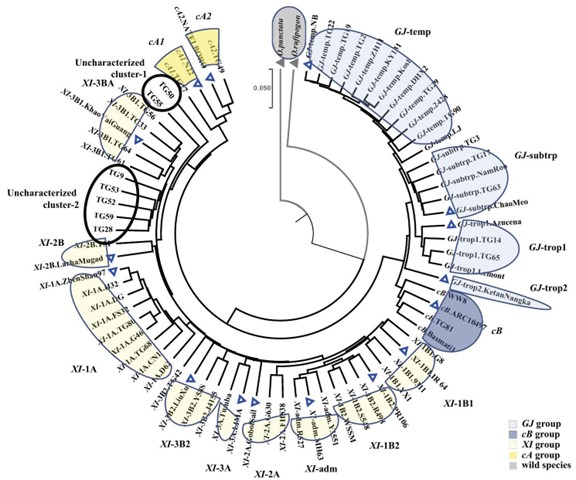
\includegraphics[width=0.8\linewidth]{figure/tree}
	\caption{使用全基因组倒位指数对75个高质量水稻基因组进行系统发育树分析} \label{tree}
\end{figure}

这部分中,研究人员使用了一些典型的数据处理方法:

\begin{enumerate}

\item UPGMA(算术平均无加权配对群组法)是一种常用的聚类方法.
它基于距离矩阵进行操作,通过计算不同样本间的成对距离,从而推断它们之间的系统发育关系.UPGMA是一种层次聚类方法,其基本思想是逐步将距离最近的样本或样本群组合并,直到所有样本都被归入一个大的群组中.


\item Mantel检验是一种数据处理方法,其计算公式如下:

$$
r=\frac{\sum_{i=1}^{n-1} \sum_{j=i+1}^n\left(X_{i j}-\bar{X}\right)\left(Y_{i j}-\bar{Y}\right)}{\sqrt{\sum_{i=1}^{n-1} \sum_{j=i+1}^n\left(X_{i j}-\bar{X}\right)^2\left(Y_{i j}-\bar{Y}\right)^2}}
$$

其中,$X_{ij}$ 和 $Y_{ij}$ 分别表示两个距离矩阵中的元素,$\bar{X}$ 和 $\bar{Y}$ 分别表示距离矩阵的平均值,$n$ 是观测值的数量.

\end{enumerate}


\subsubsection{其他分析和结果概要}
由于本报告篇幅有限,无法详细分析所有结果,以下简要概述其他部分:

\begin{enumerate}
	\item 分析了亚洲水稻及其两个野生近缘种(O. punctata和O. rufipogon)中的物种特异性、群体特异性和共享倒位.提出了特异性倒位和倒位速率的模型.
	\item 研究了水稻全基因组倒位指数中的转座子元素分布.发现三个转座子元素家族(LTR-RT Ty1-copia、Ty3-gypsy 和 DNA-TE MULE)在倒位断点处的频率较高.
	\item 分析了位于倒位断点处基因的转录丰度.展示了MH63(XI-adm)基因组中位于倒位末端的两个OsNAS基因拷贝,以及倒位对其5'UTR区域的影响.同时,研究了OsNAS基因在根组织中的转录丰度以及Fbox基因编码序列在MH63(XI-adm)中如何被倒位破坏.
	\item 对大倒位的群体连锁不平衡进行了分析.研究了倒位导致的连锁不平衡(LD)区块破坏,展示了倒位如何破坏两个LD区块.同时,给出了一个实例,说明高LD的SNP区块被倒位破坏,以及IRGSP RefSeq(GJ-temp)与Azucena(GJ-trop1)单倍型区块不连续时,INV030410区域的Azucena(GJ-trop1)单倍型区块被破坏.
\end{enumerate}

\subsubsection{基因组倒位的鉴定与评估方法}

本文的研究者旨在识别大型倒位(>100 bp),在两个基因组(GJ-temp: IRGSP-1.0 和 XIadm: MH63)上测试了四种分析流程.

工作流程1:MH63基因组切成约10倍覆盖率的50 Kb重叠片段,使用NGMLR映射到IRGSP-1.0,并用SVIM调用倒位.保留深度大于6且通过筛选标准的倒位.

工作流程2:与工作流程1类似,但使用Sniffles调用倒位.

工作流程3:MH63基因组与IRGSP-1.0使用Minimap2对齐.筛选出大于90\%同源性和长度大于100 bp的结果.使用SyRI调用倒位.

工作流程4:与工作流程3类似,但使用MUMmer的Nucmer进行对齐.

本文的研究者验证后最后选择了工作流程4,使用MUMmer将74个基因组序列与IRGSP RefSeq对齐,筛选最小90\%同源性和最小100 bp长度.用MUMmer的“showcoords”功能获取坐标.最后,使用SyRI工具调用倒位,生成包含ID、参考和查询基因组坐标起始、结束位置的VCFs,用于下游全基因组比较.

关于这部分内容,研究者开源了代码,我也尝试了在Linux系统下安装numcer,syri等软件进行序列的比对和评估测试,不过由于原文亚洲水稻基因的数据量确实比较大(一个数据集大约100多M,其实不算大,但是也不小了),暂时还没有来得及复现文章的结果,因此也不再赘述了.

\subsubsection{研究实例总结和展望}

本研究通过全面分析亚洲稻米种群结构层面的倒位变异,揭示了倒位在水稻中的重要性.倒位作为一种重要的结构变异类型,对于基因重组抑制、适应性特征选择、生殖隔离和物种形成具有显著作用.通过发现1769个非冗余倒位并估计了不同层次的倒位速率,本研究为倒位研究提供了新的见解.

展望未来,亚洲稻米泛基因组倒位指数的建立仅是揭示稻米中所有自然变异的第一步.下一步研究者将建立亚洲稻米的水稻数字基因库,将超过100,000份测序数据映射到水稻种群参考组.稻米基因组结构变异的研究和应用,将为未来稻米育种和农业发展提供支持.通过这一研究实例的学习和分析,我们也认识到泛基因组学在大规模组学数据和科学计算时代可以发挥非常重要的作用.

